\documentclass[tikz,border=2pt]{standalone}
\usepackage{amsmath}
\usetikzlibrary{arrows.meta}
\begin{document}
% Entry with unknown type: Nature draws competitive (1/5) or weak (4/5); the competitive type
% enters, the weak type enters with probability 1/2. The incumbent's information set after entry
% is reached with probabilities 0.2 and 0.4, so mu = 0.2/0.6 = 1/3 on the competitive node.
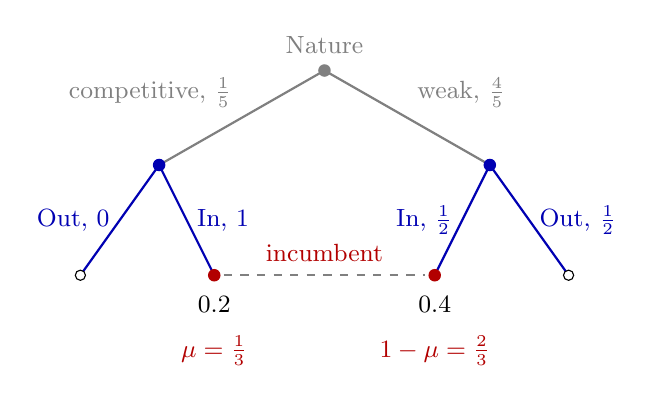
\begin{tikzpicture}[font=\small, >={Latex[length=2mm]},
    dec/.style={circle, fill, inner sep=1.6pt},
    term/.style={circle, draw, fill=white, inner sep=1.3pt}]
  % Nature
  \draw[thick, gray] (0,0) -- node[above left, pos=0.5] {competitive, $\tfrac15$} (-2.1,-1.2);
  \draw[thick, gray] (0,0) -- node[above right, pos=0.5] {weak, $\tfrac45$} (2.1,-1.2);
  % entrant's choices
  \draw[thick, blue!70!black] (-2.1,-1.2) -- node[left, pos=0.5] {Out, $0$} (-3.1,-2.6);
  \draw[thick, blue!70!black] (-2.1,-1.2) -- node[right, pos=0.5] {In, $1$} (-1.4,-2.6);
  \draw[thick, blue!70!black] (2.1,-1.2) -- node[left, pos=0.5] {In, $\tfrac12$} (1.4,-2.6);
  \draw[thick, blue!70!black] (2.1,-1.2) -- node[right, pos=0.5] {Out, $\tfrac12$} (3.1,-2.6);
  % incumbent's information set
  \draw[dashed, thick, gray] (-1.28,-2.6) -- (1.28,-2.6);
  \node[red!70!black, anchor=south] at (0,-2.55) {incumbent};
  % nodes
  \node[dec, gray, label={[gray]above:Nature}] at (0,0) {};
  \node[dec, blue!70!black] at (-2.1,-1.2) {};
  \node[dec, blue!70!black] at (2.1,-1.2) {};
  \node[dec, red!70!black] at (-1.4,-2.6) {};
  \node[dec, red!70!black] at (1.4,-2.6) {};
  \node[term] at (-3.1,-2.6) {};
  \node[term] at (3.1,-2.6) {};
  % reach probabilities and beliefs
  \node[anchor=north] at (-1.4,-2.75) {$0.2$};
  \node[anchor=north] at (1.4,-2.75) {$0.4$};
  \node[red!70!black, anchor=north] at (-1.4,-3.25) {$\mu=\tfrac13$};
  \node[red!70!black, anchor=north] at (1.4,-3.25) {$1-\mu=\tfrac23$};
\end{tikzpicture}
\end{document}
